\documentclass[tikz, preview]{standalone}
\usepackage{amsfonts, amsthm, amssymb, amsmath, stmaryrd, etoolbox}
\usepackage{tikz}
\usetikzlibrary{matrix,arrows}
\tikzset{->-/.style={decoration={markings, mark=at position .5 with {\arrow{>}}},postaction={decorate}}}
\tikzset{->-pos/.style={decoration={markings, mark=at position #1 with {\arrow{>}}},postaction={decorate}}}
\tikzset{->-/.style={decoration={markings,mark=at position .5 with {\arrow{>}}},postaction={decorate}}}
\tikzset{->-pos/.style={decoration={markings,mark=at position #1 with {\arrow{>}}},postaction={decorate}}}

\begin{document}
%%%%%%%%%%%%%%%%% 
%%%%%%%%%%%%%%%%% 
\[
  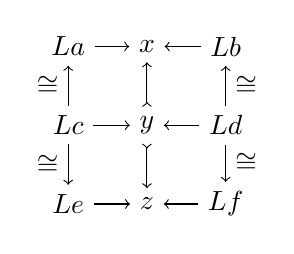
\begin{tikzpicture}
   % \draw [help lines, step=0.2, color=blue!10] (-5,-5) grid (5,5); % grid
    % 
    \node (1) at (-1,1) {$ La $};
    \node (4) at (0,1) {$ x $};
    \node (7) at (1,1) {$ Lb $};
    \node (2) at (-1,0) {$ Lc $};
    \node (5) at (0,0) {$ y $};
    \node (8) at (1,0) {$ Ld $};
    \node (3) at (-1,-1) {$ Le $};
    \node (6) at (0,-1) {$ z $};
    \node (9) at (1,-1) {$ Lf $};
    \draw [->] (1) to node [] {$  $} (4);
    \draw [->] (7) to node [] {$  $} (4);
    \draw [->] (2) to node [] {$  $} (5);
    \draw [->] (8) to node [] {$  $} (5);
    \draw [->] (3) to node [] {$  $} (6);
    \draw [->] (9) to node [] {$  $} (6);
    \draw [->] (2) to node [left] {$ \cong $} (1);
    \draw [->] (2) to node [left] {$ \cong $} (3);
    \draw [>->] (5) to node [] {$  $} (4);
    \draw [>->] (5) to node [] {$  $} (6);
    \draw [->] (8) to node [right] {$ \cong $} (7);
    \draw [->] (8) to node [right] {$ \cong $} (9);
  \end{tikzpicture}
\]
%%%%%%%%%%%%%%%%% 
%%%%%%%%%%%%%%%%% 
\end{document}
